\documentclass[10pt, conference]{IEEEtran}
\IEEEoverridecommandlockouts
\usepackage[
  backend=biber,
  maxcitenames=3,
  minbibnames=1,
  mincitenames=1,
  maxbibnames=3,
  uniquelist=false,
  style=ieee,
  url=false,
  doi=true,
  eprint=true,
]{biblatex}
\AtBeginBibliography{\footnotesize}
\addbibresource{references.bib}
\usepackage{booktabs}
\usepackage{tabularx}
\usepackage{csquotes}
\usepackage[table]{xcolor}
\usepackage{tablefootnote}
\usepackage{numprint}
\usepackage{nicematrix}
\usepackage[compat=0.6]{yquant}
\usepackage{lipsum}
\usepackage{comment}
\usepackage{tikz}
\usetikzlibrary{arrows.meta}
\usetikzlibrary{positioning,fit}
\usetikzlibrary{patterns,calc}
\usetikzlibrary{tikzmark}
\usepackage{fp}
\usepackage{xspace}
\usepackage{amsmath,amssymb,amsfonts}
\usepackage{bbm}
\usepackage{quantikz}
\usepackage{placeins}
\usepackage[T1]{fontenc}
\usepackage[colorlinks=true,urlcolor=teal,
            linkcolor=teal,citecolor=teal]{hyperref}
\usepackage[most]{tcolorbox}
\usepackage{listings}
\usepackage{censor}
\definecolor{lfd1}{HTML}{000000}
\definecolor{lfd2}{HTML}{E69F00}
\definecolor{lfd3}{HTML}{999999}
\definecolor{lfd4}{HTML}{009371}
\definecolor{lfd5}{HTML}{beaed4}
\definecolor{lfd6}{HTML}{ed665a}
\definecolor{lfd7}{HTML}{1f78b4}
\definecolor{bggray}{gray}{0.9}
\newcommand{\TODO}[1]{\textcolor{red}{TODO: #1}}

\def\chapterautorefname{Chapter}%
\def\sectionautorefname{Sec.}%
\def\subsectionautorefname{Sec.}%
\def\subsubsectionautorefname{Sec.}%
\def\paragraphautorefname{Par.}%
\def\tableautorefname{Tab.}%
\def\equationautorefname{Eq.}%
\def\figureautorefname{Fig.}%

\newcommand{\reprolink}{https://doi.org/10.5281/zenodo.13132521}
\newcommand{\ie}{\emph{i.e.}\xspace}
\newcommand{\eg}{\emph{e.g.}\xspace}
\newcommand{\etal}{\emph{et al.}\xspace}
\newcommand{\rj}{\emph{ReJoin}\xspace}
\newcommand{\repro}{\href{\reprolink}{reproduction package}\xspace}
\newcommand{\mapa}{Marcus and Papaemmanouil\xspace}

\newcommand{\atUL}[1]{\textcolor{blue}{@UL: #1}}
\newcommand{\atOTH}[1]{\textcolor{magenta}{@OTH: #1}}

\newcommand{\Ket}[1]{$\ket{#1}$}
\newcommand{\Bra}[1]{$\bra{#1}$}
\newcommand{\BraKet}[2]{$\braket{#1}{#2}$}

\makeatletter
\def\calcLength(#1,#2)#3{%
\pgfpointdiff{\pgfpointanchor{#1}{center}}%
             {\pgfpointanchor{#2}{center}}%
\pgf@xa=\pgf@x%
\pgf@ya=\pgf@y%
\FPeval\@temp@a{\pgfmath@tonumber{\pgf@xa}}%
\FPeval\@temp@b{\pgfmath@tonumber{\pgf@ya}}%
\FPeval\@temp@sum{(\@temp@a*\@temp@a+\@temp@b*\@temp@b)}%
\FProot{\FPMathLen}{\@temp@sum}{2}%
\FPround\FPMathLen\FPMathLen5\relax
\global\expandafter\edef\csname #3\endcsname{\FPMathLen}
}
\makeatother

\lstdefinestyle{query}{
  language=SQL,
  %numbers=left,
  stepnumber=1,
  numbersep=10pt,
  tabsize=4,
  showspaces=false,
  showstringspaces=false,
  basicstyle=\linespread{1}\fontfamily{lmtt}\selectfont\small,
  keywordstyle=\color{blue},
  stringstyle=\color{purple},
  upquote=true,
  breaklines=true,
  commentstyle=\color{CadetBlue}
}

\definecolor{mygray}{rgb}{0.643,0.643,0.643}
\newtcolorbox{querybox}[2][]{%
  sidebyside align=top,
  enhanced,
  boxsep=2pt,
  arc=0pt,
  top=-3pt, bottom=-3pt,
  left=2pt, right=0pt,
  colback=white,
  colframe=mygray,
  boxrule=0.5pt,
  leftrule=12pt,
  overlay unbroken and first ={%
    \node[rotate=90,
          minimum width=0.5cm,
          anchor=south,
          %font=\small\rmfamily,
          yshift=-11pt,
          white]
    at (frame.west) {#2};
  }
}

\newtcolorbox{matrixbox}[2][]{%
  sidebyside align=top,
  enhanced,
  boxsep=0pt,
  arc=0pt,
  left=-1em,
  top=-0.8em,
  boxrule=0pt,
  colframe=bggray,
  colback=bggray,
  leftrule=12pt,
  overlay unbroken and first ={%
    \node[rotate=90,
          minimum width=0.5cm,
          anchor=south west,
          font=\itshape,
          yshift=0pt, %-14pt,
          xshift=0.5em,
          black]
    at (frame.south west) {#2};
  }
}

\newcommand{\CXgate}{\ensuremath{\text{C\raisebox{0.08em}{--}}\!\hat{X}}\xspace}
\newcommand{\CYgate}{\ensuremath{\text{C\raisebox{0.08em}{--}}\!\hat{Y}}\xspace}
\newcommand{\CZgate}{\ensuremath{\text{C\raisebox{0.08em}{--}}\!\hat{Z}}\xspace}

\newcommand{\nop}[1]{}

\newlength{\WIDTH}\newlength{\HEIGHT}
\renewcommand{\Join}{\bowtie}

\newboolean{anonymous}
\setboolean{anonymous}{false}
\ifbool{anonymous}{}{\renewcommand{\censor}[1]{#1}}
\ifbool{anonymous}{}{\renewcommand{\blackout}[1]{#1}}
\ifbool{anonymous}{\newcommand{\genemail}[2]{\href{mailto:xxx.xxx@xx.xx}{\blackout{#2}}}}{\newcommand{\genemail}[2]{\href{#1}{#2}}}

\begin{document}
\title{Supplementary Material -- Hype or Heuristic? Quantum Reinforcement Learning for Join Order Optimisation}

\author{\IEEEauthorblockN{\blackout{Maja Franz}}
\IEEEauthorblockA{\blackout{\textit{Technical University of}}\\
    \blackout{\textit{Applied Sciences Regensburg}} \\
    \blackout{Regensburg, Germany} \\
    \genemail{mailto:maja.franz@othr.de}{maja.franz@othr.de}}
\and
\IEEEauthorblockN{\blackout{Tobias Winker}}
\IEEEauthorblockA{\blackout{\textit{University of Lübeck}}\\
    \blackout{Lübeck, Germany}\\
    \genemail{mailto:t.winker@uni-luebeck.de}{t.winker@uni-luebeck.de}}
\and
\IEEEauthorblockN{\blackout{Sven Groppe}}
\IEEEauthorblockA{\blackout{\textit{University of Lübeck}}\\
    \blackout{Lübeck, Germany}\\
    \genemail{mailto:sven.groppe@uni-luebeck.de}{sven.groppe@uni-luebeck.de}}
\and
\IEEEauthorblockN{\blackout{Wolfgang Mauerer}}
\IEEEauthorblockA{\blackout{\textit{Technical University of}}\\
    \blackout{\textit{Applied Sciences Regensburg}}\\
    \blackout{\textit{Siemens AG, Technology}}\\
    \blackout{Regensburg/Munich, Germany}\\
    \genemail{mailto:wolfgang.mauerer@othr.de}{wolfgang.mauerer@othr.de}}
}

\maketitle

\begin{abstract}
  This document provides additional information and experiments conducted for the paper \enquote{Hype of Heuristic? Quantum Reinforcement Learning for Join Order Optimisation}.
\end{abstract}

\section{Introduction}
\label{sec:intro}
In particular, we address the following:
\begin{enumerate}
  \item We provide an outline of the replication of the classical reinforcement learning (RL) approach by \mapa~\cite{marcus18} for the join order (JO) problem in \autoref{sec:exp-crl}.
  \item The process of finding good hyperparameters for each setting is described in \autoref{sec:hyper}. We also list the parameters, which lead to the training runs depicted in the main study.
\end{enumerate}

\section{Classical Baseline Replication}
\label{sec:exp-crl}

While the main study focuses on the experimental results of the quantum-based version of \rj, this section is an extension of Sec.~IV-C (methodology of the multistep QRL approach) and Sec.~VB (experimental results) in the main study with a focus on the classical baseline replication.

\subsection{Methodology}

\subsubsection{Classical Model}
As in the original study~\cite{marcus18}, we utilise two fully-connected NNs, one for the actor-part and one for the critic part of PPO, using two hidden layers with 128 units each.

\subsubsection{Training and Test Data}
For classical \rj, we trained and evaluated the model using 113 queries from the join order benchmark (JOB).
We applied a ten-fold cross-validation scheme~\cite{fushiki2011}, whereby the dataset is split into ten distinct parts. Each part is excluded from the training set once to be utilised for testing, leading to ten different train-test-splits.
While \rj\cite{marcus18} selects ten test queries for evaluation and the remaining 103 queries for training on a random basis, we adopt ten-fold cross-validation, which is a commonly accepted to demonstrate generalisability~\cite{goodfellow16}.

As discussed in the main study, we also conduct experiments on a limited number of relations in a query, resulting in fewer queries in the dataset.
Similar to Krishnan~\etal~\cite{krishnan18}, we generate new queries based on subplans to enlarge the dataset.
However, instead of obtaining subplans from the traditional optimiser, we rely on a single \rj training run, generating over \numprint{12000} subqueries.
Note that the newly generated dataset is not used in our classical baseline replication experiments described in this supplementary material, but in the main study.

\subsubsection{Setting the Join Order}
To specify the selected join order for the \emph{PG} cost model, we utilise the \texttt{pg\_hint\_plan}~\cite{pg_hint_plan} extension that allows to control the execution plan of a query with hinting phrases.
A join order can then be selected using RL, and the rest of the query plan choices are left to the traditional optimiser\footnote{%
  For our replication of Ref.~\cite{marcus18}, we relied on explicit join clauses~\cite{postgres} using PostgreSQL V8.4, as in the original study}.


\subsubsection{Reward Signal}
\label{sec:single-step-reward}
In the original study~\cite{marcus18}, the agent is rewarded with zero for each intermediate step and with the reciprocal of the final join order's cost, that is, $R_{t}^{(\text{rec})} = \frac{1}{C_{\text{RL}}^{(\text{CM})}}$ in the final timestep $T$ of an episode.
Here, $C_{\text{RL}}^{(\text{CM})}$ represents the costs assigned to the join order selected by the RL agent according to the cost model CM.
Since we initially achieved a subpar training convergence for $R_t^{(\text{rec})}$, inspired by the implementation of another RL technique for JO, \emph{RTOS}~\cite{rtos_impl}, we used a different reward signal in our experiments:
\begin{equation}
  R_t^{(\text{mrc})} = -\min\left[\log_{10}\left(\frac{C_{\text{RL}}^{(\text{CM})}}{C_{\text{DP}}^{(\text{CM})}} + 1\right), 4\right] + \log_{10}(2) + 1
\end{equation}
where $C_{\text{DP}}^{(\text{CM})}$ is the cost of the best join order determined by a dynamic programming (DP) exhaustive search according to cost model CM.
The logarithm allows for expressing a large range of costs and additionally clipping the ratio to be at most $4$ and shifting it with $log_{10}(2) + 1$ to be at most $1$ reduces the chances of steeper gradients during training, which is a known problem that can lead to suboptimal training~\cite{laud03}.

\subsubsection{Cost Models}
We investigate the influence of two different cost models:

\paragraph{PG}
The first model is the default cost model of PostgreSQL~\cite{postgres}\footnote{For our baseline comparison, we use PostgreSQL V8.4 to ascertain compatibility with the original experimental setting, while V16.0 is utilised in subsequent experiments.}, which calculates a cost estimate for a selected JO and its correspondence query plan based on metadata, such as cardinalities and selectivities.
PostgreSQL's built-in optimiser also uses these costs estimates to select a JO.
However, because of errors in cost estimation, a selected JO is not necessarily optimal, even when using an exhaustive search based on DP.
Additionally, since DP is resource-intensive, PostgreSQL switches from DP to a genetic optimiser for queries exceeding twelve relations per default.
In the case of using (Q)ML for the JO selection, the complete query plan is established by sending the resulting JO to the PostgreSQL optimiser, which chooses the remaining optimisation decisions, such as whether to apply a hash or nested-loop join.
Lastly, the PostgreSQL cost model assigns a cost to the resulting plan.
Note that the \emph{PG} cost model is mainly considered for comparability with the original study and is not used for our quantum-based approach in the main study.

\paragraph{OUT}
To evaluate the selected join order, we use the established cost function $C_{\text{out}}$~\cite{cluet95}, which considers the cardinalities (\ie the number of tuples in a query result set) as an approximation of query complexity:
%
\begin{equation}
  C_{\text{out}}(T) =
    |T| + C_{\text{out}}(T_1) + C_{\text{out}}(T_2),
\end{equation}
%
where $n$ is the maximum number of joins in the query, a join tree is defined as $T = T_1 \Join T_2$, and $|T|$ represents the true cardinality of $T$ ($C_{\text{out}}(T) = 0$ if $T \in \{r_1, r_2, \dots\}$ is a leaf).
To obtain the optimal join orders for this reference cost model, we compute $C_{\text{out}}$ for all possible orders (excluding cross joins) and select one with the lowest cost.
Due to the high resource requirements of DP, we
start with the join order suggested by PostgreSQL for more than 
twelve joins, and update it whenever a better order is
found during training.

\subsection{Results}
\begin{figure}
  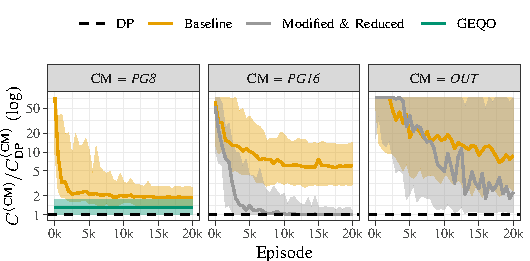
\includegraphics{img-gen/convergence_rejoin_base.pdf}\vspace*{-0.5em}
  \caption{Relative costs over all queries in the JOB during training of re-implemented baseline and the modified/reduced version of \rj using the cost models of PostgreSQL V8.4 (\emph{PG8}) and V16.0 (\emph{PG16}), as well as $C_{\text{out}}$ (\emph{OUT}). The models were trained according to ten-fold cross-validation, such that each query is in a test-set once. We executed PostgreSQL V8.4's genetic optimiser \emph{GEQO} on every query in the JOB. The solid lines represents the medians, the areas corresponds to the first and third quartiles. To improve the visual display, results exceeding a value of 75 are cut off.}
  \label{fig:rejoin-cl}
\end{figure}

Our attempt at replicating the approach and experiments of Ref~\cite{marcus18} are illustrated on the left of \autoref{fig:rejoin-cl}.
Despite some minor deviations from the findings in Ref.~\cite{marcus18}, which claim that \rj can on average reach 20\% cheaper plans than PostgreSQL's genetic optimiser \emph{GEQO} on the test dataset after approximately \numprint{10000} sampled episodes, we believe that our results constitute a successful effort of replicating \rj.
The evaluation of our replication confirms that \rj can learn near-optimal join orders, similar to \emph{GEQO}, and even match the optimal orders of DP in some cases.
The deviations from the original results could possibly be attributed to differing hyperparameters or settings.
As unfortunately the hyperparameters are not specified in Ref.~\cite{marcus18}, we conducted an extensive hyperparameter search, for which individual runs and the resulting parameters can be found in \autoref{sec:hyper}.
Nevertheless, we cannot guarantee exact agreement with the original study.

\subsection{Baseline Modifications}\label{sec:mod}
To further enhance the outcomes of our replication, and to allow for the reduced encoding described in the main study in Par. IV-C2a, we combined methods from other RL approaches for JO~\cite{krishnan18, xiang20} to improve the learning convergence in cost training.

\subsubsection{Incorporating Orders from the Traditional Optimiser}
\label{subsec:mod-trad}

In our previous evaluations of our replication, we found that throughout the whole training process, actions were sampled for certain queries, resulting in suboptimal rewards and therefore in join orders leading to high costs.
This indicates that the model may have become trapped in a local optimum.
To address this, we select actions in the sampling stage of PPO based on the join order selected for a specific query by the traditional optimiser, which is easily obtainable and near-optimal.
A similar technique is utilised in Ref.~\cite{krishnan18}, which is based on Q-learning, an RL approach that assimilates knowledge from stored experience in a \emph{replay buffer}, from which is sampled to train the model.
To pre-fill this buffer, Krishnan~\etal employ (sub-)join orders that occur in the query plan of the traditional optimiser.
As a replay buffer is not present in PPO, we sample actions from the traditional optimiser's join orders with probability $p_{O} \in [0, 1]$ in the sampling stage; $p_{O}$ requires hyperparameter tuning.

\subsubsection{Updating the Training Dataset based on Rewards}
\label{subsec:mod-update}
As mentioned above, basic \rj fails to find good join orders for specific queries.
One possibility for learning better join orders for these \enquote{hard} queries is to increase the amount of samples taken.
Ref.~\cite{xiang20} adds multiple copies of a \enquote{hard} query to the training set based on the reward associated with the join order that can be achieved with the current policy.
We update the training dataset every $s_U \in [0, s_{\text{max}}]$ episodes, where $s_{\text{max}} \in \mathbb{N}$ is the maximum number of sampled episodes.
In the update, a copy of each query achieving a reward below the threshold $th_U \in \mathbb{R}$ is added to the training dataset. This introduces hyperparameters $s_U$ and $th_U$.

\subsubsection{Multi-Step Reward Signal}
\label{subsec:mod-multistep}

In previous studies on RL for JO (\eg, Refs.~\cite{krishnan18, marcus18, xiang20}) the reward, as function of cost, is only assigned at the end of each episode when the full join order is built by the RL policy. Intermediate steps receive a zero reward.
This seems counter-productive, given that one property of RL is to determine an action based on a current state and reward signal.
Assuming the cost difference $C_t^{(\text{CM})}$ between timesteps $t$ and $t-1$ with costs $c_k$ for subtrees $T_k \in \mathcal{F}$ in a state $S_t$ according to cost model CM is
\begin{equation}
  C_t^{(\text{CM})} = 
  \begin{cases}
    \sum_{T_k \in \mathcal{F}} c_k - C_{t-1}^{(\text{CM})} & \text{if } t > 0 \\
    0 & \text{if } t = 0
  \end{cases},
\end{equation}
and the cost assigned to the order of the full query determined by DP is $C_{\text{DP}}^{(\text{CM})}$, we propose the clipped reward at $t$ as
\begin{equation}
  R_t^{(\text{mult})} = \frac{1}{n-1} \left[-\min\left(\frac{C_t^{(\text{CM})}}{C_{\text{DP}}^{(\text{CM})}}, n-1 \right) + 2\right].
\end{equation}

This requires $(n-1)$ joins (and actions) to build the join tree for a query with $n$ relations.
As for $R_t^{(\text{mrc})}$, shifting and normalising reduces the chance for steep gradients.
We introduce whether the multi-step or single-step reward signal (cf. \autoref{sec:single-step-reward}) should be used as an additional hyperparameter.

The experiments involving the application of modifications and reduction of input feature space, as discussed in Par. IV-C2a in the main study, were conducted using PostgreSQL V16.0's cost model due to its compatibility with the \texttt{pg\_hint\_plan} extension. This extension facilitates simpler manipulation of join plans than explicit join clauses.
The outcomes of the modified and reduced \rj, as well as the baseline \rj on the two cost models \emph{PG}, with PostgreSQL V16.0, and \emph{OUT} are depicted in \autoref{fig:rejoin-cl}\footnote{To assure a fair comparison, we used a similar number of parameters for both, the full and the reduced \rj versions, resulting in two fully-connected layers with each 128 or 384 hidden units, respectively.}.
According to the figure, the modified and reduced \rj version can achieve lower costs than the baseline, with considerably fewer input components.
This confirms that the reduced \rj can serve as classical basis for subsequent QRL calculations.
Furthermore, we observed that training convergence is particularly sensitive to hyperparameters.
For example, in our top-performing test of the baseline version in PostgreSQL V8.4, we utilised a low learning rate (\ie optimiser step-size) of 8e-5.
However, costs for \emph{OUT} using the modified version significantly varied with this rate, and we settled on a learning rate of 3e-4
(cf.~\autoref{sec:hyper} for hyperparameters for all configurations).
Despite various efforts to find similar optimal hyperparameters for the \emph{OUT} cost-model, both configurations are less stable in training.
Higher costs for \emph{OUT} compared to \emph{PG} may be a reason for this observation.
The maximum relative costs across all experiments in \autoref{fig:rejoin-cl} were about 330 times higher for \emph{OUT} than for \emph{PG}.
By clipping the calculated reward signal, we avoid steep gradients and retain small median costs for the modified and reduced version.
Yet significant variations in cost range leave several outliers.

\section{Hyperparameter Search}
\label{sec:hyper}

\begin{table*}
  \caption{Hyperparameters subject to search.}
  \label{tab:hyperparams}

  \definecolor{lightgray}{gray}{0.95}
  \rowcolors{3}{lightgray}{}

  \begin{tabularx}{\textwidth}{llXl}
    \toprule
    \rowcolor{white} \textbf{Hyperparameter} & \textbf{Variable name} & \textbf{Description} & \textbf{Possible values} \\
    \midrule
    $p_O$ & \texttt{take\_best\_threshold} & Probability of sampling optimal actions from the traditional optimiser (modified \rj only, cf.~\autoref{subsec:mod-trad}). & \{ 0.1, 0.2, 0.5 \} \\
    $s_U$ & \texttt{take\_best\_frequency} & Number of episodes after which to update the dataset based on rewards (modified \rj only, cf.~\autoref{subsec:mod-update}). & \{ 10, 50, 100, 500, \numprint{1000} \} \\
    $th_U$ & \texttt{update\_dataset\_reward\_threshold} & Threshold, below which rewards are added to the train set every $s_U$ episodes (modified \rj only, cf.~\autoref{subsec:mod-update}). & \{ -1, 0, 0.5 \} \\
    $\eta_\text{start}$ & \texttt{lr\_start} & Initial value for the learning rate. & \{ 5e-5, 8e-5, 9e-5, 1e-4, 2e-4, 3e-4 \} \\
    $\eta_\text{duration}$ & \texttt{lr\_duration} & Share of the training process for which the learning rate decays linearly until a learning rate of 1e-8 is reached. A value of zero corresponds to no decay in the learning rate. & \{ 0, 0.5, 0.9 \} \\
    multistep reward & \texttt{multistep} & Whether to use a multi-step (modified \rj only, cf.~\autoref{subsec:mod-multistep}) or single-step (cf.~\autoref{sec:single-step-reward}) signal. & \{ True, False \} \\
    $n_\text{episodes}$ & \texttt{batchsize} & Number of episodes per batch in PPO (cf. Ref.~\cite{schulman17}). & \{ 5, 10, 20, 50, 100 \} \\
    \bottomrule
  \end{tabularx}
\end{table*}

All training runs undertaken in this study underwent a comprehensive hyperparameter search.
To achieve this, hyperparameters were fine-tuned in four steps:
\begin{enumerate}
  \item Firstly, we determined hyperparameters of interest and a possible selection of values, listed in \autoref{tab:hyperparams}.
  \item As testing over \numprint{8000} combinations of hyperparameters in a grid search is too extensive, we randomly selected 50 of all configurations on the specified training and test dataset in Ref.~\cite{marcus18}\footnote{For the training runs in the main study on four relations, we conducted the initial hyperparameter search on the first train-test split} for each cost model (\emph{PG8}, \emph{PG16}, \emph{OUT}) and setting (Baseline, Modified \& Reduced).
.
  \item  While we can not guarantee that we identified the best hyperparameter constellation, as we were only able to test a part of the possible constellations, we collected the four most efficient hyperparameter combinations, meaning those that resulted in the lowest average costs over the last three validation steps. These top-performing combinations were subsequently utilised for the 10-fold cross-validation.
  \item Finally, we selected the combination with the lowest average costs over the last three validation steps and all queries in the test sets as the optimal one.
\end{enumerate}

The final parameters for each configuration are listed in \autoref{tab:final-params}. The raw results can also be found in this corresponding \repro.
\begin{table*}
  \caption{Final hyperparameter values for the training results in this supplementary material and in the main study.}
  \label{tab:final-params}

  \definecolor{lightgray}{gray}{0.95}
  \rowcolors{3}{lightgray}{}

  \begin{tabularx}{\textwidth}{llllX}
    \toprule
    \rowcolor{white} \textbf{Configuration} & \textbf{Cost model} & \textbf{Results} & \textbf{Hyperparameter} & \textbf{Value} \\
    \midrule
    Classical -- Baseline & \emph{PG8} & \autoref{fig:rejoin-cl}, left & & \\
    & & & $\eta_\text{start}$ & 9e-5 \\
    & & & $\eta_\text{duration}$ & 0.9 \\
    & & & $n_\text{episodes}$ & 20 \\
    \midrule
    Classical -- Baseline & \emph{PG16} & \autoref{fig:rejoin-cl}, mid & & \\
    & & & $\eta_\text{start}$ & 9e-5 \\
    & & & $\eta_\text{duration}$ & 0.9 \\
    & & & $n_\text{episodes}$ & 20 \\
    \midrule
    Classical -- Modified \& Reduced & \emph{PG16} & \autoref{fig:rejoin-cl}, mid & & \\
    & & & $p_O$ & 0.1 \\
    & & & $s_U$ & 1 \\
    & & & $th_U$ & 0.5 \\
    & & & $\eta_\text{start}$ & 3e-4 \\
    & & & $\eta_\text{duration}$ & 0.9 \\
    & & & multistep reward & False \\
    & & & $n_\text{episodes}$ & 20 \\
    \midrule
    Classical -- Baseline & \emph{OUT} & \autoref{fig:rejoin-cl}, right & & \\
    & & & $\eta_\text{start}$ & 5e-5 \\
    & & & $\eta_\text{duration}$ & 0.9 \\
    & & & $n_\text{episodes}$ & 20 \\
    \midrule
    Classical -- Modified \& Reduced & \emph{OUT} & \autoref{fig:rejoin-cl}, right & & \\
    & & & $p_O$ & 0.1 \\
    & & & $s_U$ & 1 \\
    & & & $th_U$ & 0.5 \\
    & & & $\eta_\text{start}$ & 3e-4 \\
    & & & $\eta_\text{duration}$ & 0.9 \\
    & & & multistep reward & False \\
    & & & $n_\text{episodes}$ & 20 \\
    \midrule
    Quantum \& Classical -- Modified \& Reduced -- Four Relations & \emph{OUT} & Main study, Figs. 5 \& 6 & & \\
    & & & $p_O$ & 0.1 \\
    & & & $s_U$ & 1 \\
    & & & $th_U$ & 0.5 \\
    & & & $\eta_\text{start}$ & 3e-4 \\
    & & & $\eta_\text{duration}$ & 0.9 \\
    & & & multistep reward & True \\
    & & & $n_\text{episodes}$ & 20 \\
    \bottomrule
  \end{tabularx}
\end{table*}


\newcommand{\MF}{\censor{MF}\xspace}
\newcommand{\WM}{\censor{WM}\xspace}
\newcommand{\TW}{\censor{TW}\xspace}
\newcommand{\SG}{\censor{SG}\xspace}
\newcommand{\programme}{\blackout{German Federal Ministry of
Education and Research (BMBF), funding program \enquote{Quantum Technologies---from
Basic Research to Market}}}
\newcommand{\grantsoth}{\censor{\#13N15647 and \#13NI6092}}
\newcommand{\grantuzl}{\censor{\#13N16090}}
\newcommand{\hta}{\blackout{High-Tech Agenda Bavaria}}

\begin{small}
\noindent\textbf{Acknowledgements} \MF, \TW, \SG and \WM were supported by
the \programme, grants \grantsoth\ (\MF and \WM), and \grantuzl\ (\TW and \SG).
\WM acknowledges support by the \hta.
\end{small} 

\printbibliography

\end{document}
